\documentclass{article}
\usepackage{a4wide}
\usepackage[utf8]{inputenc}
\usepackage{amsmath}
\usepackage{mathtools}
\usepackage{amssymb}
\usepackage[english]{babel}
\usepackage{mdframed}
\usepackage{systeme,}
\usepackage{lipsum}
\usepackage{relsize}
\usepackage{graphicx}
\usepackage{caption}
\usepackage{tikz}
\usepackage{tikz-3dplot}
\usepackage{pgfplots}
\usepackage{harpoon}%
\usepackage{graphicx}
\usepackage{wrapfig}
\usepackage{subcaption}
\usepackage{a4wide}
\usepackage{comment}
\usepackage{authblk}
\usepackage{float}
\usepackage{listings}
\usepackage{xcolor}
\usepackage{amsmath}
\usepackage{chngcntr}
\usepackage{amsthm}
\usepackage{comment}
\usepackage{commath}
\usepackage{hyperref}%Might remove, adds link to each reference
\usepackage{url}
\newcommand{\w}{\omega}
\newcommand{\curl}[1]{\vec{\nabla}\times \vec{#1}}
\newcommand{\grad}{\vec{\nabla}}
\newcommand{\dive}[1]{\vec{\nabla}\cdot \vec{#1}}
%\newcommand{\crr}{\mathfrak{r}}
\usepackage{calligra}

\DeclareMathAlphabet{\mathcalligra}{T1}{calligra}{m}{n}
\DeclareFontShape{T1}{calligra}{m}{n}{<->s*[2.2]callig15}{}
\newcommand{\crr}{\mathcalligra{r}\,}
\newcommand{\boldscriptr}{\pmb{\mathcalligra{r}}\,}

\title{Handin4 FK7048}
\author{Author : Andreas Evensen}
\date{Date: \today}
\definecolor{codegreen}{rgb}{0,0.6,0}
\definecolor{codegray}{rgb}{0.5,0.5,0.5}
\definecolor{codepurple}{rgb}{0.58,0,0.82}
\definecolor{backcolour}{rgb}{0.95,0.95,0.92}

\lstdefinestyle{mystyle}{
    backgroundcolor=\color{backcolour},   
    commentstyle=\color{codegreen},
    keywordstyle=\color{magenta},
    numberstyle=\tiny\color{codegray},
    stringstyle=\color{codepurple},
    basicstyle=\ttfamily\footnotesize,
    breakatwhitespace=false,         
    breaklines=true,                 
    captionpos=b,                    
    keepspaces=true,                 
    numbers=left,                    
    numbersep=5pt,                  
    showspaces=false,                
    showstringspaces=false,
    showtabs=false,                  
    tabsize=2
}

\lstset{style=mystyle}

\begin{document}

\maketitle

\section*{Warm up problems}

\subsection*{a)}
Suppose the following PDE:
\begin{align*}
    y'' = x^2 + 4.
\end{align*}We wish to solve this with Greens functions with the boundary-conditions $y(0) = y'(L)=0$; thus we can rewrite the above equation to the following:
\begin{align*}
    y'' = f(x); \quad f(x) = x^2 + 4.
\end{align*}We thus wish to find the Greens function $G(x,s)$ such that:
\begin{align*}
    y(x) &= \int_0^x G_1(x,s)f(s)ds + \int_{x}^L G_2(x,s)f(s)ds\\
    &=\int_0^x (-s) f(s)ds + \int_{x}^L (-x)f(s)ds\\
    &= \left[-\frac{s^4}{4} - 2s^2\right]_0^x - x\left[\frac{s^3}{3} + 4s\right]_x^L\\
    &= -\Big[\frac{x^4}{4} + 2x^2\Big] - x\Big[\frac{L^3}{3} + 4L - \frac{x^3}{3} -4x\Big]\\
    &= 2x^2 + \frac{x^4}{12} - \Big[\frac{xL^3 + 12xL}{3}\Big]
\end{align*}

\subsection*{b)}
We wish to find a general seperable solution to the following PDE:
\begin{align*}
    \frac{\partial u}{\partial t} - \lambda \frac{\partial^2 u}{\partial x^2} = 0.
\end{align*}We thus assume that $u$ can be decomposed in the following manner:
\begin{align*}
    u(x,t) &= X(x)T(t)\\
    \implies \frac{T'}{T}& = \lambda\frac{X''}{X} = c = \mu^2.
\end{align*}With this we can assume the following, since $\lambda > 0$:
\begin{align}
    T(t) &= c_1\exp\big[-\frac{\lambda}{\mu^2}t\big] + c_2\nonumber\\
    X(x) &= A\cos(\frac{x}{\mu}) + B\sin\big(\frac{x}{\mu}\big)\nonumber\\
    \implies u(x,t) &= e^{-\frac{\lambda}{\mu^2} t}\Big(\tilde{A}\cos(\frac{x}{\mu}) + \tilde{B}\sin(\frac{x}{\mu})\Big)\label{eq 1.2 sol}
\end{align}We test this solution by inserting it into the PDE:
\begin{align*}
   &\frac{\partial}{\partial t} \Bigg[e^{-\frac{\lambda}{\mu^2} t}\Big(\tilde{A}\cos(\frac{x}{\mu}) + \tilde{B}\sin(\frac{x}{\mu})\Big)\Bigg] - \lambda \frac{\partial^2}{\partial x^2}\Bigg[e^{-\frac{\lambda}{\mu^2} t}\Big(\tilde{A}\cos(\frac{x}{\mu}) + \tilde{B}\sin(\frac{x}{\mu})\Big)\Bigg]\\
   &=-\frac{\lambda}{\mu^2} e^{-\frac{\lambda}{\mu^2} t}\Big(\tilde{A}\cos(\frac{x}{\mu}) + \tilde{B}\sin(\frac{x}{\mu})\Big) + \frac{\lambda}{\mu^2} e^{-\frac{\lambda}{\mu^2} t}\Big(\tilde{A}\cos(\frac{x}{\mu}) + \tilde{B}\sin(\frac{x}{\mu})\Big) = 0.
\end{align*}Thus eq \eqref{eq 1.2 sol} is a solution to the PDE, we now find the constants by the initial-condtions:
\begin{align*}
    u(0, t) &= e^{-\frac{\lambda}{\mu^2} t}\Big(\tilde{A}\Big) = 0\implies \tilde{A} = 0.\\
    u(L, t) &= e^{-\frac{\lambda}{\mu^2} t}\Big(\tilde{B}\sin\big(\frac{L}{\mu}\big)\Big) = 0\implies \mu = \frac{n\pi}{L}, \quad n = 0,1,2,3,\dots\\ 
\end{align*}Thus the final solution for the PDE is the following:
\begin{align*}
    u_n(x,t) &= \tilde{B}\exp\left[-\frac{\lambda\cdot L^2}{\Big(n\pi\Big)^2}\right]\sin\left(\frac{x\cdot L}{n\pi}\right)
\end{align*}

\section*{Laplace equation}
Suppose the following PDE:
\begin{align}
    &\frac{1}{r^2}\frac{\partial^2}{\partial r^2}\Big(r^2\frac{\partial \phi}{\partial r}\Big) + \frac{1}{r^2\sin(\theta)}\frac{\partial}{\partial \theta}\Big(\sin(\theta)\frac{\partial \phi}{\partial \theta}\Big) + \frac{1}{r^2\sin^2(\theta)}\frac{\partial^2\phi}{\partial \varphi^2}=0,\label{eq: 2.1}\\
    &u_r(R, \theta) = 0; \quad \forall\theta\in[0,\pi],\nonumber
\end{align} where $\phi= \phi(\rho, z)$. Given a slip condition we have the following boundary-conditions:
\begin{align*}
    u_r(R, \theta) =0;\quad \forall\theta\in[0,\pi].
\end{align*}Moreover, we recall Laplace's equation:
\begin{align*}
    0 &=\left[\frac{d^2}{dx^2} + \frac{d^2}{dy^2}+\frac{d^2}{dz^2}\right]u\quad \text{In cartesian coordinates}
\end{align*}
\subsection*{a)}
We wish to find boundary condtion for $r\to \infty$ such that $\mathbf{u} = U\hat{z}$ in polar coordinates, i.e we wish to find the following functions, $\alpha(\theta)$ and $\beta(\theta)$ such that the following holds:
\begin{align*}
    \lim_{r\to\infty}\mathbf{u}(r, \theta) &= U\left[\alpha(\theta)\hat{r} + \beta(\theta)\hat{\theta}\right] = U\hat{z}\\
\end{align*}We recall that the unit-vectors can be written as, when treating the $y$ component as zero:
\begin{align*}
   \hat{r} &= \cos(\theta)\hat{z} + \sin(\theta)\hat{x},\\
   \hat{\theta} &= \cos(\theta)\hat{x}-\sin(\theta)\hat{z}.
\end{align*}Hence, we have two equations, one for the $\hat{x}$ direction and one for $\hat{z}$ direction. This thus implies $\alpha(\theta) = \cos(\theta)$ and $\beta(\theta) = -\sin(\theta)$.

\subsection*{b)}
Suppose the following function to be a solution to the PDE \eqref{eq: 2.1}:
\begin{align*}
    \phi(r, \theta) = A\cdot r\cos(\theta) + \frac{B}{r}+\frac{C\cos(\theta)}{r^2}.
\end{align*}
We wish to find the constants $A$, $B$ and $C$ by the boundary-conditions implied by eq \eqref{eq: 2.1}, and the limit condition defined above. In order to do so, we first compute the 
gradient of the function $\phi(r, \theta)$, where the $\varphi$ component is zero:
\begin{align*}
    \vec{\nabla}\phi(r, \theta)&=\Bigg[\frac{\partial}{\partial r}\Big(Ar\cos(\theta) + \frac{B}{r}+\frac{C\cos(\theta)}{r^2}\Big)\hat{r}+\frac{1}{r}\frac{\partial}{\partial \theta}\Big(Ar\cos(\theta) + \frac{B}{r}+\frac{C\cos(\theta)}{r^2}\Big)\hat{\theta}\Bigg]\\
    &=\left[\Big(A\cos(\theta) - \frac{B}{r^2} - \frac{2C\cos(\theta)}{r^3}\Big)\hat{r}-\Big(A\sin(\theta) +\frac{C\sin(\theta)}{r^3}\Big)\hat{\theta}\right]
\end{align*}
If we look at the $\hat{r}$ component we have by the boundary-conditions that:
\begin{align*}
    \hat{r}\cdot\vec{\nabla}\phi(R, \theta) &=A\cos(\theta) - \frac{B}{R^2} - \frac{2C\cos(\theta)}{R^3} = 0\\
    \implies &\cos(\theta)\Big(\underbrace{A-\frac{2C}{R^3}}_{=0}\Big)= 0\quad \forall\theta\in[0,\pi]
\end{align*}Thus we have that $B = 0$ and $A = \frac{2C}{R^3}$, we now use the second boundary-condition:
\begin{align*}
    \lim_{r\to\infty} \vec{\nabla}\phi &= U\hat{z}\\
    \implies \lim_{r\to\infty} \cdot\vec{\nabla}\phi&=\lim_{r\to\infty}\left[\frac{\hat{z}}{\cos(\theta)}\Big(A\cos(\theta) - \frac{C\cos(\theta)}{2r^3}\Big)\right]\\
    &\lim_{r\to\infty}\Big[A-\frac{B}{2r^3}\Big]\hat{z} = U\hat{z}.
\end{align*}Thus we have that $A = U$, and $C = \frac{1}{2}UR^3$. Moreover, this is a valid solution to the PDE posed in eq \eqref{eq: 2.1}, which has a physical interpretation of a static field with both a monopole and a dipole contribution; however the monopole contribution is zero.

\subsection*{c)}
The velocity field is given by $\mathbf{u}(r, \theta)$, which thus is given by the gradient of $\phi(r, \theta)$:
\begin{align*}
    \mathbf{u}(r, \theta) &= \vec{\nabla}\phi(r, \theta) =\left[\Big(U\cos(\theta) - \frac{UR^3\cos(\theta)}{r^3}\Big)\hat{r}-\Big(U\sin(\theta) +\frac{UR^3\sin(\theta)}{2r^3}\Big)\hat{\theta}\right]
\end{align*}
\begin{figure}[H]
    \centering
    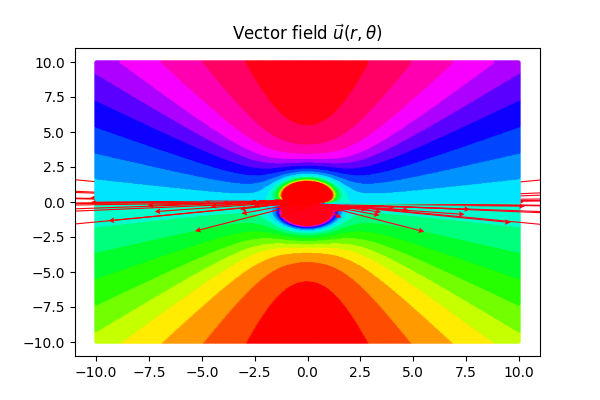
\includegraphics[scale =0.5]{task2_3.png}
    \caption{The velocity field $\mathbf{u}$}
    \label{fig: 2.3}
\end{figure}\noindent
The velocity field $\mathbf{u}$ shows that the velocity becomes constant as $r$ grows, which was in accordane to our boundary-conditions. Moreover, it's expanding around a singularity point which also is to be expected. It symmetric around $\hat{\theta}$ which also is to be expected from a physical perspective.

\section*{Wave equation}
Suppose the following PDE;
\begin{align*}
    \frac{\partial^2u}{\partial t^2} &= c^2\frac{\partial^2w}{\partial x^2}\\
    \text{Initial-conditions: }&\begin{cases}
        u(x,0) = q(x)\\
        \frac{\partial u}{\partial t}(x,0) = p(x)
    \end{cases};\quad \forall x\in\mathbb{R}.
\end{align*}It has a solution to the initial value problem, given by:
\begin{align}
    u(x,t) &=\frac{1}{2}\Big(q(x+ct) + q(x - ct)\Big)+\frac{1}{2c}\int_{x - ct}^{x + ct}p(s)ds\label{eq 3.1}
\end{align}

\subsection*{a)}
Given the following definitions of $p(x)$ and $q(x)$:
\begin{align*}
    \begin{cases}
        q(x) &= \Big(1-\frac{\abs{x}}{L}\Big)H\Big(1-\frac{\abs{x}}{L}\Big)\\
        p(x) &=0
    \end{cases},
\end{align*}where $H(x)$ is the Heaviside operator. In the function \eqref{eq 3.1}, we analyse the integral given the functions $q(x)$, and $p(x)$ defined above:
\begin{align*}
    u(x,t) &= \frac{1}{2}\Bigg[\Big(1-\frac{\abs{x + ct}}{L}\Big)H\Big(1-\frac{\abs{x + ct}}{L}\Big) + \Big(1-\frac{\abs{x - ct}}{L}\Big)H\Big(1-\frac{\abs{x - ct}}{L}\Big)\Bigg]\\
    &+\frac{1}{2}\int_{x - ct}^{x + ct}0ds\\
    u(x,t) &= \frac{1}{2}\Bigg[\Big(1-\frac{\abs{x + ct}}{L}\Big)H\Big(1-\frac{\abs{x + ct}}{L}\Big) + \Big(1-\frac{\abs{x - ct}}{L}\Big)H\Big(1-\frac{\abs{x - ct}}{L}\Big)\Bigg]\\
\end{align*}
\begin{figure}[H]
    \centering
    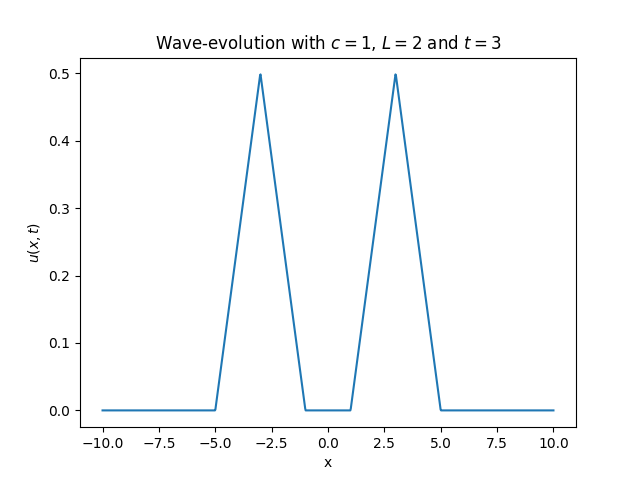
\includegraphics[scale = 0.5]{task3_1.png}
    \caption{Time-evolution of the propagating wave}
    \label{fig: 3.1}
\end{figure}\noindent
As seen in the figure above, the wave propagates with a velocity $c$ in both directions of the origin, $x_0 = 0$. I wont lose amplitude as it propagates in time, but rather the amplitude is constant.
The physical meaning of this is a wave propagating through a medium without friction, e.g vaccum.

\subsection*{b)}
Given the following definitions of $p(x)$ and $q(x)$:
\begin{align*}
    \begin{cases}
        q(x) &= 0\\
        p(x) &= H(x+L)H(L-x)
    \end{cases}.
\end{align*}Using these definitions in the function \eqref{eq 3.1}, yields the following:
\begin{align*}
    u(x,t) &= \frac{1}{2}\Big(0\Big) + \frac{1}{2c}\int_{x-ct}^{x+ct}d\tilde{x}\Big[H(\tilde{x} + L)H(L - \tilde{x})\Big]\\
    &=\frac{1}{2c}\Bigg[(\tilde{x}+L)H(\tilde{x}+L)H(L-\tilde{x}) + 2 L H(\tilde{x}-L)\Bigg]_{\tilde{x} = x-ct}^{\tilde{x} = x+ct}\\
\end{align*}

\begin{figure}[H]
    \centering
    \begin{subfigure}[b]{0.45\textwidth}
        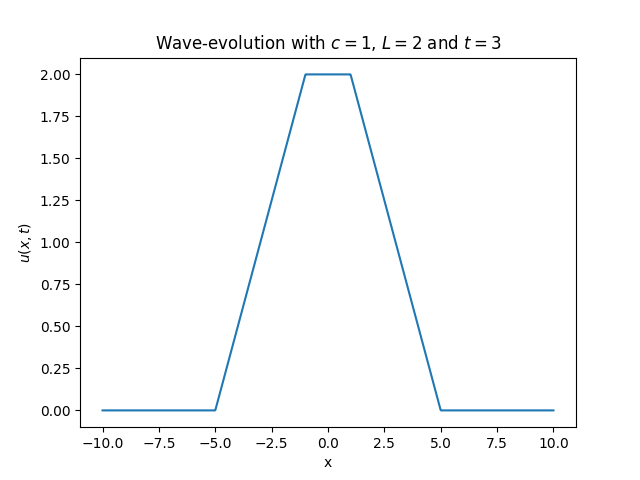
\includegraphics[scale = 0.4]{task3_2.png}
        \caption{Wave propagating at $t = 3$ .}
        \label{fig:3_2_1}
    \end{subfigure}
    \hfill
    \begin{subfigure}[b]{0.45\textwidth}
        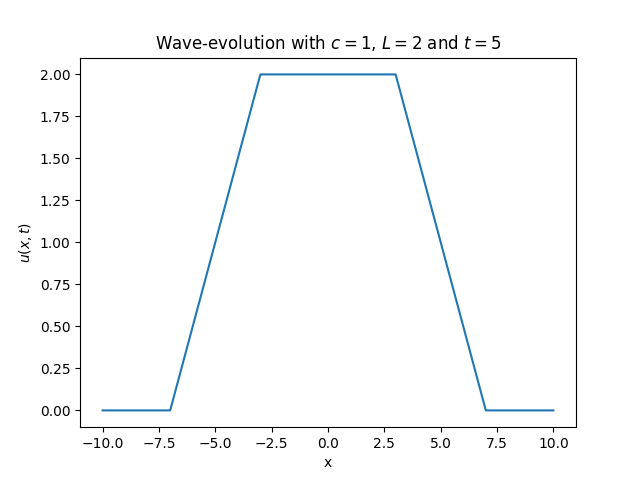
\includegraphics[scale = 0.4]{task3_2_2.png}
        \caption{Wave propagating at $t = 5$ .}
        \label{fig:3_2_2}
    \end{subfigure}
    \caption{Time-evolution of the wave}
\end{figure}\noindent
Again the amplitude does not change when time increases but rather the extent of the wave increases. In time it would reach a steady state of which has a constant ampltiude extending, for $t\to\infty$ for all $x\in\mathbb{R}$.

\subsection*{Proving the primitive function}
In order to prove the primitive function of the Heaviside operator, we recall the following identity:
\begin{align*}
    \delta(x) = \frac{d}{dx}\Big(H(x)\Big).
\end{align*}Taking the derivative of the primitiv-function yields:
\begin{align*}
    \frac{d}{dx}\big(g(x)\big) &=\frac{d}{dx}\Big[(x + L)H(x + L)H(L-x)\Big] + \frac{d}{dx}\Big[2LH(x-L)\Big]\\
    &=H(x+L)H(L-x) + (x+L)H'(x+L)H(L-x) - H(x+L)H'(L-x)\\
    &+2LH'(x-L)\\
    &= H(x+L)\Big(H(L-x) - H'(L-x)\Big) + (x+L)H'(x+L)H(L-x) + 2LH'(x-L)\\
    &= H(x+L)\Big(H(L-x) - \underbrace{\delta(L-x)}_{=0}\Big) + \underbrace{(x+L)\delta(x+L)H(L-x)}_{=0} + \underbrace{2L\delta(x-L)}_{=0}\\
    &= H(x+L)H(L-x).
\end{align*}

\subsubsection*{c)}
As seen by the figures above: fig \ref{fig: 3.1} and \ref{fig:3_2_1}, there is a difference between the two waves. The first waves propagates through space as a transversing wave, while the second wave propagates through space and accumulates
the amplitude. One can be seen as plucking a string, the first wave, whilst the second wave can be viewed as a wave that leaves a transvering trace through space.
\\
\\
This can be viewed by eq \eqref{eq 3.1}, since the second wave is just the ingral of the expression for $p(x)$. Thus the second wave can be viewed as a super-position of many small waves, which in turn have a constant amplitude.

\end{document}
    